\documentclass[10pt]{article}
\usepackage[utf8]{inputenc}
\usepackage[english]{babel} % The automatic words such as Table, Figure, ... appear in the specified language


% To define non-default page margins
\usepackage[left=2.5cm, right=3cm]{geometry}

\usepackage{hyperref} % Hyperlinks


\usepackage{tikz} % Plots, Graphs, ...
\usetikzlibrary {arrows.meta} % For the Latex style arrow


\usepackage{graphicx}
% \usepackage{subcaption}

\usepackage{listings} % to write code

\usepackage{float} % For figure placement option H

% Math
\usepackage{amsmath} % math
\usepackage{amsfonts} % For for example \mathbb{}

% Tables
\usepackage{tabularx} 
\usepackage{multicol}
\usepackage{multirow}


% Macros
\newcommand{\N}{\mathbb{N}}




\title{Workshop \LaTeX\,Cheat Sheet}
\author{João Dionísio and Manuel Lamas}
\date{December 2022}


\begin{document}

\maketitle

\section{Introduction}

What is \LaTeX?
\begin{itemize}
    \item It differentiates itself from Word and Libre Office because it is not a WYSIWYG (What you see is what you get) system. This means that we have a source code file that does not represent the end result. We visualize the PDF in a separate viewer.
    \item Several functionalities can be added via packages, which can be installed (and then included in each specific file) as the need arises.
\end{itemize}

This document is organized as follows: Section $2$ is dedicated to math expressions, Section $3$ to text formatting, Sections $4$ and $5$ to images and tables respectively, and Section $6$ to plotting and graph drawing with Ti$k$Z. The document ends with some miscellaneous commands and useful links.

This document is organized as follows: \hyperref[sec:math]{Section 2} is dedicated to math expressions, \hyperref[sec:text_format]{Section 3} to text formatting, \hyperref[sec:images]{Sections 4} and \hyperref[sec:tables]{5} to images and tables respectively, and \hyperref[sec:tikz]{Section 6} to plotting and graph drawing with Ti$k$Z. The document ends with \hyperref[sec:misc]{Section 7} with some miscellaneous commands and useful links.

\section{Math Expressions}
\label{sec:math}

\LaTeX is very often used as a typesetting language for mathematics, due to its ease of use. To write simple expressions, we just need to write them in between dollar signs, like so: $1+1=2$. If we do not wish to write the math expression inline, we can also use double dollar signs:

$$x = y + 3$$

Furthermore, we can get more control if we use the equation environment, from the \verb|amsmath| package.

\begin{equation}
    \sum_{i=1}^{\infty}\dfrac{1}{n^{2}} = \dfrac{\pi^{2}}{6}
    %\caption{Basel problem's equation}
    \label{eq:basel_problem}
\end{equation}

With environments such as these, we can then refer to specific equations, such as Equation~\ref{eq:basel_problem}.
To be able to do so we need to define a label within the environment through the \verb|\label|, which is then used in the \verb|\ref| command.


Fractions can be easily written using the \verb|\dfrac{}{}| command, as seen in the example above. The command also requires the \verb|amsmath| package. Further math commands can be easily found online, for example at \href{https://en.wikibooks.org/wiki/LaTeX/Mathematics}{Wikibooks}. 


\section{Text Formatting}
\label{sec:text_format}

It can be useful to format the text, and the standard ways of doing so are readily available: \textbf{bold}, \emph{emphasize}, \underline{underline}. To do a linebreak, both the command \verb|\linebreak| and the command \verb|\\| do the same thing\footnote{Also, this is how to create a footnote.}.\\
% There are two commands for italicizing a word https://tex.stackexchange.com/a/26934
There are some nuances when using \LaTeX. For example, if we wish to use quotation marks, we must start the expression with two grave accents and end it with two apostrophes. "Wrong" and ``Right''. Also, we need to be careful with special characters in text, as they need to be prefixed by a backslash: $10\%$.

We can also create lists, with the itemize command:

\begin{itemize}
    \item Where we can write
    \item $x\times y = 1$
\end{itemize}

And with the enumerate command, the items are numbered:

\begin{enumerate}
    \item One
    \item Zwei
    \item Trois
\end{enumerate}

% Furthermore, we can also use \verb|\pagebreak| if we wish to jump to the next page, like so \pagebreak


\section{Insert Images}
\label{sec:images}

With the graphicx package, inserting images is straightforward.

\includegraphics[width = .3\textwidth]{Images/Cardioid.png}

Using the~\verb|\includegraphics[]{}| command, we can control the images' size with the square brackets, and the image itself goes in the curly brackets. If we create a folder to store the images (which is a good practice to have an organized workspace), then the directory has to be included. In our example, we have a file ``Cardiod.png'' in the Images folder. So we need to use \verb|Images/Cardioid.png|. To center the image, we have the \verb|\centering| command.

As with math expressions and the equation environment, images also have an environment that allows us to have more control over them. For example, we can specify the position of the figure. The standard options are h, t, b, and p, which stand respectively for here, top, bottom, and page of floats. They mean that the figure should be placed exactly where it is written in the text, at the top of the next page, at the bottom of the next page, and in a page of floats, separate from the text. These options can sometimes be ignored by \LaTeX, but if one really wants them to be enforced, using ``!h'' instead of just ``h'' may be able to override this.
For more on this topic see \href{https://en.wikibooks.org/wiki/LaTeX/Floats,_Figures_and_Captions#Figures}{placement specifier parameter}.

\begin{figure}[ht]
    \centering % Centers horizontally
    \includegraphics[width = .3\textwidth]{Images/Cardioid.png}
    \caption{A beautiful caption for a beautiful cardioid.}
    \label{fig:cardioid}
\end{figure}

Just like we did for equation, we can also refer to a specific figure, for example, figure~\ref{fig:cardioid}. Some of these environments also allow us to provide a caption, through the \verb|\caption| command.

Notice that we use \verb|~| in-between figure and its reference, the tilde creates a ``non-breaking space'' meaning it creates a space that cannot be affected by a line break. 





\section{Tables}
\label{sec:tables}

Aside from what we presented, we can also create tables. Like with math expressions and graphics, we can use the \verb|\tabular| environment from the \verb|tabularx| package for creating a simple table, but it is generally preferable to use \verb|\table|, also due to the greater control over the tabular.

Horizontal lines are added with \verb|\hline|, and the number of columns and placement of vertical lines are defined when beginning the tabular. For example, \verb_\begin{tabular}{|c c | c|}_, assuming everything else is completed correctly, defines a table with $3$ columns and vertical lines before the first column, between the second and the third, and after the third column.

\begin{table}[h]
    \centering
    \begin{tabular}{|c|c|c|c|c|}
          \hline
         $\times$ & \textbf{1} & \textbf{i} & \textbf{j} & \textbf{k} \\
          \hline
        \textbf{1} & 1 & i & j & k \\
          \hline
        \textbf{i} & i & -1 & -k & -j \\
          \hline
        \textbf{j} & j & -k & -1 & i \\
          \hline
        \textbf{k} & k & j & -i & -1 \\
          \hline
    \end{tabular}
    \caption{Quaternion multiplication table}
    \label{tab:quaternions}
\end{table}

In table~\ref{tab:quaternions_modified} we present a modified version of the table~\ref{tab:quaternions}.
We removed horizontal lines by removing two \verb|\hline| commands, as well as some vertical lines by changing the tabular parameter given when beginning the tabular environment \verb_\begin{tabular}{c|cc|c|c}_. % https://tex.stackexchange.com/questions/10629/escape-in-verb


\begin{table}[h]
    \centering
    \begin{tabular}{c|cc|c|c}
        \hline
         $\times$ & \textbf{1} & \textbf{i} & \textbf{j} & \textbf{k} \\

        \textbf{1} & 1 & i & j & k \\
        \hline
        \textbf{i} & i & -1 & -k & -j \\
        \hline
        \textbf{j} & j & -k & -1 & i \\

        \textbf{k} & k & j & -i & -1 \\
        \hline
    \end{tabular}
    \caption{Quaternion multiplication table (modified)}
    \label{tab:quaternions_modified}
\end{table}


More advanced tables can be created using the commands \verb|\multirow| and \verb|\multicolumn|, which require the packages \verb|multirow| and \verb|multicol|.

\begin{table}[h!]
    \centering
    \begin{tabular}{ |c|c|c|c| }
    	\hline
    	\multirow{2}{*}{Test} & \multicolumn{3}{c|}{Note Code} \\
    	\cline{2-4}
    	& A & B & C \\
    	\hline
    	-1 & 0 & 1 & 2 \\
    	\hline
    	0 & 12 & 13 & 14 \\
    	\hline
    	1 & 24 & 25 \\
        \cline{0-2}
    \end{tabular}
    \caption{Testing a table with some peculiarities}
    \label{tab:table_multi} % Must be after the caption
\end{table}



\section{Tikz}
\label{sec:tikz}

\paragraph*{TikZ example} The \verb|tikz| package allows us to plot functions like the one in figure~\ref{fig:tikz_example}. But it can also be used to create graphs, as the one in figure~\ref{fig:graph}, and many other kinds of diagrams. See more on the webpage \href{https://tikz.dev/}{Ti$k$Z}.

\begin{figure}[ht]
    \centering
    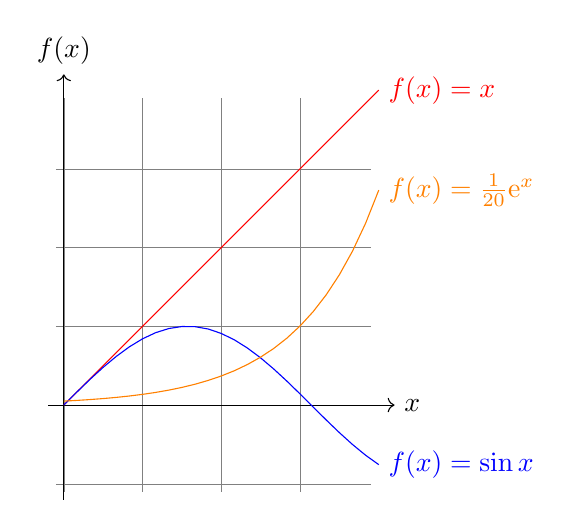
\begin{tikzpicture}[domain=0:4]
      \draw[very thin,color=gray] (-0.1,-1.1) grid (3.9,3.9);
    
      \draw[->] (-0.2,0) -- (4.2,0) node[right] {$x$};
      \draw[->] (0,-1.2) -- (0,4.2) node[above] {$f(x)$};
    
      \draw[color=red]    plot (\x,\x)             node[right] {$f(x) =x$};
      % \x r means to convert '\x' from degrees to _r_adians:
      \draw[color=blue]   plot (\x,{sin(\x r)})    node[right] {$f(x) = \sin x$};
      \draw[color=orange] plot (\x,{0.05*exp(\x)}) node[right] {$f(x) = \frac{1}{20} \mathrm e^x$};
    \end{tikzpicture}
    \caption{Plotting functions with the Ti$k$Z package.}
    \label{fig:tikz_example}
\end{figure}


\begin{figure}
    \centering
    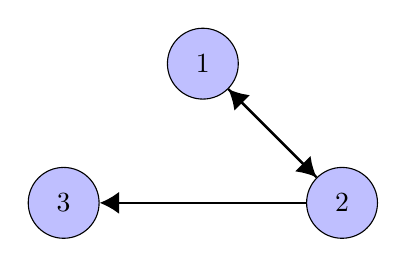
\begin{tikzpicture}[node distance = 2.5cm, minimum size = 0.9cm,
    	main/.style = {draw, circle, fill = blue!25},
    	edge/.style = {->, line width = 0.8pt, arrows = {-Latex[width = 8pt, length = 7pt]}}]
    	\node[main] (1) {$1$};
    	\node[main] (2) [below right of=1] {$2$};
    	\node[main] (3) [below left of=1] {$3$};
    	\draw (1)[edge] -- (2);
    	\draw (2)[edge] -- (1);
    	\draw (2)[edge] -- (3);
    \end{tikzpicture}
    \caption{A Graph made with Ti$k$Z}
    \label{fig:graph}
\end{figure}


\section{Miscellaneous}
\label{sec:misc}

\paragraph{Comments:}
Comments can be added with a \verb|%| (percentage symbol), anything written after one will be ignored and not presented in the resulting PDF, remaining present in the source code only.
% This line will only be visible in the source code file

\paragraph{Hyperlinks:}
For adding hyperlinks, as we have been using throughout the text, we use the \verb|\href| command.
It requires the \verb|hyperref| package
An example of a hyperlink for more information on the subject of \href{https://en.wikibooks.org/wiki/LaTeX/Hyperlinks}{Hyperlinks}.


\paragraph*{Macros:}
One can create commands to achieve a large number of effects. One of the most commonly used is to facilitate the usage of other commands that are frequently used. For example, to replace the command \verb|\mathbb{N}|, we can create a command \verb|\N| adding the following in the preamble \verb|\newcommand{\N}{\mathbb{N}}|. And then we can simply use $\N$.

This example serves as a simple illustration, we would not usually create macros that are essentially copies of other commands.
But instead, we would use it for longer and more detailed commands that we use often.

\paragraph*{Resources:}
\begin{itemize}

    \item \href{https://www.texstudio.org/}{TeXstudio} is our recommendation to start playing around with \LaTeX;
    \item \href{https://www.overleaf.com/}{Overleaf} is a good tool for collaborative work (especially in real-time);
    \item \href{https://www.learnlatex.org/en/}{Learn \LaTeX} is a well-structured website for in-depth learning of how \LaTeX works.
\end{itemize}




\end{document}